Grovers Suchalgorithmus lässt sich so anpassen, dass er auch auf ähnliche verwandte Probleme angewandt werden kann.
Bisher wurde für den Algorithmus vorausgesetzt, dass $\mathbf{f}$ genau ein Element $\mathbf{\hat x}$ auf $\mathbf{1}$ abbildet und die anderen Elemente auf $\mathbf{0}$. 
Diese Voraussetzung ist aber nicht bei jeder Suche gegeben. In den folgenden Abschnitten werden Suchalgorithmen betrachtet, bei denen es mehr als eine korrekte Lösung und unbekannt viele Lösungen gibt. 
Abschließend wird in Abschnitt x die Suche nach dem Minimum betrachtet. 

\subsection{Suche nach einer von mehreren Lösungen}

Angenommen in der Menge der möglichen Lösungen $\mathbf{N}$ befindet sich nicht nur ein Element $\mathbf{\hat x}$, welches $\mathbf{f}$ auf $\mathbf{1}$ abbildet, sondern mehrere. 
Bei der Suche mit einem klassischen Computer verringert sich die Anzahl der Auswertungen von $\mathbf{f(x)}$ entsprechend der Anzahl der vorhandenen Lösungen. So würde bei vier korrekten Lösungen in $\mathbf{N}$ nur noch ein Viertel der ursprünglichen Auswertungen zu erwarten sein.
Auch bei der Quantensuche verringert sich der Aufwand entsprechend, ohne eine große Modifizierung am Algorithmus vorzunehmen.
Für die Suche nach einer von mehreren Lösungen ist wieder ein Orakel $\mathbf{U \textsubscript{f}}$ gegeben, wobei die Funktion $\mathbf{f}$ genau $\mathbf{k}$ Elemente $\mathbf{\hat x \textsubscript{1}}$, ..., $\mathbf{\hat x \textsubscript{k}}$ auf $\mathbf{1}$ abbildet. $\mathbf{k}$ ist somit die bekannte Anzahl der Lösungen in $\mathbf{N}$, mit $\mathbf{N = 2^n}$. 
Der Algorithmus besteht wieder aus den folgenden Schritten:
\begin{quote}
    \begin{enumerate}
        \item \textbf{Superpositionen aufbauen}
        \\
        Es wird die gleichverteilte Superposition aufgebaut, indem alle Qubits in die Superposition gebracht werden:
        \\
        \begin{equation}
            R \leftarrow H\textsubscript{n} |0 ... 0\rangle 
        \end{equation}
        \item \textbf{Amplitudenveränderung durchführen}
        \\
        Grover-Iteration auf $\mathbf{R}$ anwenden und so die Amplitudenveränderungen durchführen. Die Grover-Iteration wird dabei $\mathbf{G(N,k)}$-mal ausgeführt.
        \\
        \begin{equation}
            R \leftarrow -H\textsubscript{n} R\textsubscript{N} H\textsubscript{n} V\textsubscript{f} |x\rangle
        \end{equation}
        \item \textbf{Messen}
        \\
        Das Quantenregister $\mathbf{R}$ wird gemessen und die Ergebnisse ausgegeben.
    \end{enumerate}
\end{quote}

Der einzige Punkt, in dem sich dieser Algorithmus von dem ursprünglichen Grover-Algorithmus unterscheidet, ist im 2. Schritt die Anzahl der Grover-Iteration. 
Im Regelfall wird die Grover-Iteration $\mathbf{T = \frac{\pmb\pi}{4} \times \sqrt{N}}$ durchgeführt. $\mathbf{G(N,k)}$ ist jedoch definiert mit:
\\
\begin{equation}
    {G(N,k) \thickapprox \frac{\pi}{4} \times \sqrt{\frac{N}{k}}}
\end{equation}
\\
Damit reduziert die Anzahl der vorhandenen Lösungen in $\mathbf{N}$ die Anzahl der benötigten Grover-Iterationen. 
Für den Fall, dass $\mathbf{k \geq \frac{3}{4} \times N}$ kann ein zufälliges Element $\mathbf{x}$ aus $\mathbf{N}$ gewählt und $\mathbf{f(x)}$ ausgewertet werden. 
Mit einer 75 prozentigen Wahrscheinlichkeit wird $\mathbf{f(x) = 1}$ auswerten.
\\
LAUFZEIT

\subsection{Suche nach unbekannt vielen Lösungen}
Eine größere Herausforderung stellt die Suche dar, wenn im Vorhinein nicht bekannt ist, wie viele Lösungen in der durchsuchten Menge $\mathbf{N}$ vorhanden sind. 
Bisher wurde die Anzahl der Lösungen benötigt, um die Anzahl der Grover-Iterationen zu bestimmen, damit durch die Amplitudenveränderung mit großer Wahrscheinlichkeit das gesuchte Element gefunden wird. 
Ist die Anzahl der richtigen Elemente vorher nicht bekannt, so muss die Anzahl der Iterationen auf eine andere Weise bestimmt werden. 
Dazu wurde der Grover-Algorithmus von Boyer, Brassard, Høyer und Tapp weiterentwickelt und wird dementsprechend als G-BBHT Suche bezeichnet.
Wie bei der Suche nach einer von mehreren Lösungen ist ein Orakel $\mathbf{U \textsubscript{f}}$ gegeben, mit der Funktion $\mathbf{f}$, die genau $\mathbf{k}$ Elemente $\mathbf{U \textsubscript{f}}$ gegeben, wobei die Funktion $\mathbf{f}$ genau $\mathbf{k}$ Elemente $\mathbf{\hat x \textsubscript{1}}$, ..., $\mathbf{\hat x \textsubscript{k}}$ auf $\mathbf{1}$ abbildet und die restlichen Elemente auf $\mathbf{0}$. $\mathbf{N}$ ist wieder gegeben durch $\mathbf{N = n^2}$, allerdings ist dieses mal nicht bekannt wie groß $\mathbf{k}$ ist. Der angepasste Algorithmus läuft folgendermaßen ab:
\begin{quote}
    \begin{enumerate}
        \item \textbf{Superpositionen aufbauen}
        \\
        Ein zufälliges Element $\mathbf{x}$ wird aus $\mathbf{N}$ ausgewählt. Wenn $\mathbf{f(x) = 1}$ auswertet wurde erfolgreich eins der gesuchten Elemente gefunden und es kann an dieser Stelle gestoppt werden. 
        \\
        Hintergrund ist, dass $\mathbf{k \geq \frac{3}{4} \times N}$ sein könnte und in diesem Fall mit großer Wahrscheinlichkeit auch ohne Iterationen ein korrektes Ergebnis erreicht werden kann. Wertet $\mathbf{f(x) = 0}$ aus, dann wird im 2. Schritt fortgefahren.
        \item \textbf{Superpositionen aufbauen}
        \\
        Es wird ein zufälliger Wert $\mathbf{r}$ ausgewählt mit $\mathbf{r \in \{ 1, ..., \sqrt{N} \}}$. Dieses $\mathbf{r}$ bestimmt die Anzahl der Iterationen im 4. Schritt.
        \item \textbf{Superpositionen aufbauen}
        \\
        Es wird die gleichverteilte Superposition aufgebaut, indem alle Qubits in die Superposition gebracht werden:
        \begin{equation}
            R \leftarrow H\textsubscript{n} |0 ... 0\rangle 
        \end{equation}
        \item \textbf{Amplitudenveränderung durchführen}
        \\
        Die Grover-Iteration wird $\mathbf{r}$-mal auf $\mathbf{R}$ angewandt und so die Amplitudenveränderungen durchgeführt:
        \begin{equation}
            R \leftarrow -H\textsubscript{n} R\textsubscript{N} H\textsubscript{n} V\textsubscript{f} |x\rangle
        \end{equation}
        \item \textbf{Messen}
        \\
        Das Quantenregister $\mathbf{R}$ wird messen und $\mathbf{f(x)}$ für das ausgegebene Ergebnis $\mathbf{x}$ ausgewertet. Wertet $\mathbf{f(x) = 1}$ aus, so wurde eins der gesuchten Elemente gefunden und es kann an dieser Stelle gestoppt werden. Wertet $\mathbf{f(x) = 0}$ aus, so wird wieder beim 1. Schritt begonnen.
    \end{enumerate}
\end{quote}

Aus der Veröffentlichung von Boyer, Brassard, Høyer und Tapp geht hervor, dass bei Anwendung dieses Algorithmus nach einem Durchlauf eine Lösung mit einer Wahrscheinlichkeit von 25\% gefunden wurde. 
Trotz der zufällig gewählten Anzahl von Iterationen beträgt die Laufzeit für diesen Algorithmus LAUFZEIT.
Boyer, Brassard, Høyer und Tapp beschreiben eine weitere Modifizierung des Algorithmus, die es erlaubt die Laufzeit auf O LAUFZEIT zu senken. 
Dazu wird vor Beginn des Algorithmus ein $\mathbf{\pmb\lambda \in \{1, ..., \frac{4}{3} \} }$ gewählt und $\mathbf{m = 1}$ initialisiert. Die Anzahl der Iterationen $\mathbf{r}$ wird dann im 2. Schritt nicht mehr aus $\mathbf{\{1, ..., \sqrt{N}\}}$ gewählt, sondern aus $\mathbf{\{0, ..., m\}}$. 
Wertet $\mathbf{f(x)}$ im 5. Schritt dann zu $\mathbf{0}$ aus, wird $\mathbf{m}$ mit dem Faktor $\mathbf{\pmb\lambda}$ multipliziert, sodass bei dem nächsten Durchlauf des Algorithmus im 2. Schritt $\mathbf{e}$ aus $\mathbf{\{0, ..., \pmb\lambda \times m\}}$  gewählt wird. 
Im schlechtesten Fall wird so lange keine Lösung gefunden, dass $\mathbf{\pmb\lambda \times m > \sqrt{N}}$ gilt. Dann wird im 2. Schritt $\mathbf{r}$ wieder zufällig aus $\mathbf{\{0, ..., \sqrt{N}\}}$ gewählt, bis der Algorithmus terminiert. [QUELLE]


\subsection{Suche nach dem Minimum}
Bei den bisherigen Suchen wurde nur eine lokale Eigenschaft der Elemente berücksichtigt: handelt es sich bei dem aktuellen Element um jenes, welches gesucht wird. 
Vollkommen unabhängig von den anderen Elementen, die sich in $\mathbf{N}$ befinden. Bei der Suche nach dem Minimum ist jedoch eine globale Eigenschaft ausschlaggebend: Ist dieses Element kleiner, als alle anderen Elemente aus dem Feld.
Zur Lösung dieses Problems haben 1996 Dürr und Høyer basierend auf der G-BBHT Suche weiter gearbeitet und den folgenden Algorithmus entwickelt: 

Gegeben ist ein Orakel $\mathbf{U}$, welches auf ein Feld $\mathbf{T[0], ..., T[N-1]}$ zugreift. 
Dieses dient als Eingabe des Algorithmus, während das kleinste Element aus diesem Feld die Ausgabe des Algorithmus darstellt. $\mathbf{N}$ ist wieder gegeben durch $\mathbf{2^n}$. 
Für das Orakel werden zwei Quantenregister $\mathbf{|x\rangle}$ und $\mathbf{|y\rangle}$ der Länge $\mathbf{n}$, sowie ein Hilfsbit $\mathbf{|h\rangle}$ verwendet:

U formel und f formel
\begin{quote}
    \begin{enumerate}
        \item \textbf{Superpositionen aufbauen}
        \\
        Schrankenindex wählen
        Zu Beginn wird ein Anfangswert $\mathbf{j}$ für den Schrankenindex zufällig aus $\mathbf{0 \leq j \leq N-1}$ ausgewählt. Dieser wird genutzt, um das Register $\mathbf{|y\rangle}$ zu initialisieren: 
        \begin{equation}
            |y\rangle \leftarrow |j\rangle
        \end{equation}
        \item \textbf{Superpositionen aufbauen}
        \\
        Nach Dürr und Høyer werden die folgenden Schritte wiederholt, bis die Gesamtlaufzeit $\mathbf{22,5 \times \sqrt{N} + 1,4 \times \pmb\log\textsubscript{2}N^2}$ überschreitet [QUELLE]. 
        Anschließend wird mit Schritt 2. c) fortgefahren:
        \\
        \begin{enumerate}
            \item \textbf{Superpositionen aufbauen}
            \\
            Es wird die gleichverteilte Superposition aufgebaut, indem alle Qubits in die Superposition gebracht werden:
            \begin{equation}
                |x\rangle \leftarrow H\textsubscript{n}|0 ... 0 \rangle
            \end{equation}
            \item \textbf{G-BBHT Suche}
            \\
            Auf dem Register $\mathbf{|x\rangle}$ wird mit dem Quantenorakel $\mathbf{U}$ die G-BBHT Suche ausgeführt. 
            So wird aus allen Elementen des Feldes eines zufällig ausgewählt, welches kleiner als der Schrankenindex $\mathbf{T[y]}$ ist.
            \item \textbf{$\mathbf{|x\rangle}$ Messen}
            \\
            Das Quantenregister $\mathbf{|x\rangle}$ wird gemessen. 
            Gilt für das daraus resultierende Ergebnis $\mathbf{i}$, dass $\mathbf{T[i] < T[y]}$, dann 
            \begin{equation}
                |y\rangle \leftarrow |i\rangle
            \end{equation}
        \end{enumerate}

        \item \textbf{$\mathbf{|y\rangle}$ Messen}
        \\
        Abschließend wird das Register $\mathbf{|y\rangle}$ gemessen und das ausgegebene Ergebnis ist das kleinste Element des Feldes.
    \end{enumerate}
\end{quote}

Der Algorithmus ist auf den ersten Blick, insbesondere durch die Verwendung der G-BBHT Suche, recht abstrakt. 
Abbildung \ref{fig:sucheMinimumVisualisierung} soll das Verständnis durch eine vereinfachte, grafische Darstellung des Vorgehens vereinfachen. 
Der Datensatz in der Abbildung enthält hier beispielhaft die Werte $\mathbf{\{1, ..., 18\}}$, welche sich unsoriert im Feld befinden. Für die Verständlichkeit sind diese in der Abbildung jedoch aufsteigend sortiert.
\\
Zunächst wird im 1. Schritt der anfängliche Schrankenindex $\mathbf{j = 13}$ zufällig gewählt und das Register $\mathbf{|y\rangle \leftarrow |j\rangle}$ initialisiert. 
Im 2. Schritt des Algorithmus würde das Quantenorakel $\mathbf{U}$ für alle Wert $\mathbf{< 13}$ zu $\mathbf{1}$ auswerten, für alle $\mathbf{< 13}$ zu $\mathbf{0}$.
In Schritt 2. b) wird durch die G-BBHT Suche zufällig ein Element $\mathbf{T[i]}$ ausgewählt, welches kleiner als das aktuelle Element $\mathbf{T[y]}$ ist. 
In Abbildung \ref{fig:sucheMinimumVisualisierung} handelt es sich dabei um das Element $\mathbf{T[9]}$.
Da $\mathbf{T[9] < T[13]}$ und somit kleiner als der aktuelle Schrankenindex ist, wird dieses Element im Schritt 2. c) in das Register $\mathbf{|y\rangle}$ geschrieben.
Der Algorithmus startet wieder am Beginn des 2. Schrittes. In Schritt 2. b) wird wieder ein zufälliges Element durch die G-BBHT Suche ausgewählt, überprüft ob dieses kleiner als der aktuelle Schrankenindex ist und anschließend in Schritt 2. c) in das Register $\mathbf{|y\rangle}$ geschrieben.
Am Ende der Abbildung ist das Register $\mathbf{|y\rangle}$ mit dem Element $\mathbf{T[4]}$ gefüllt und der Algorithmus würde weitergeführt werden, bis das kleinste Element in dem Register $\mathbf{|y\rangle}$ steht.
\begin{figure}[hbtp]
	\centering
	\fbox{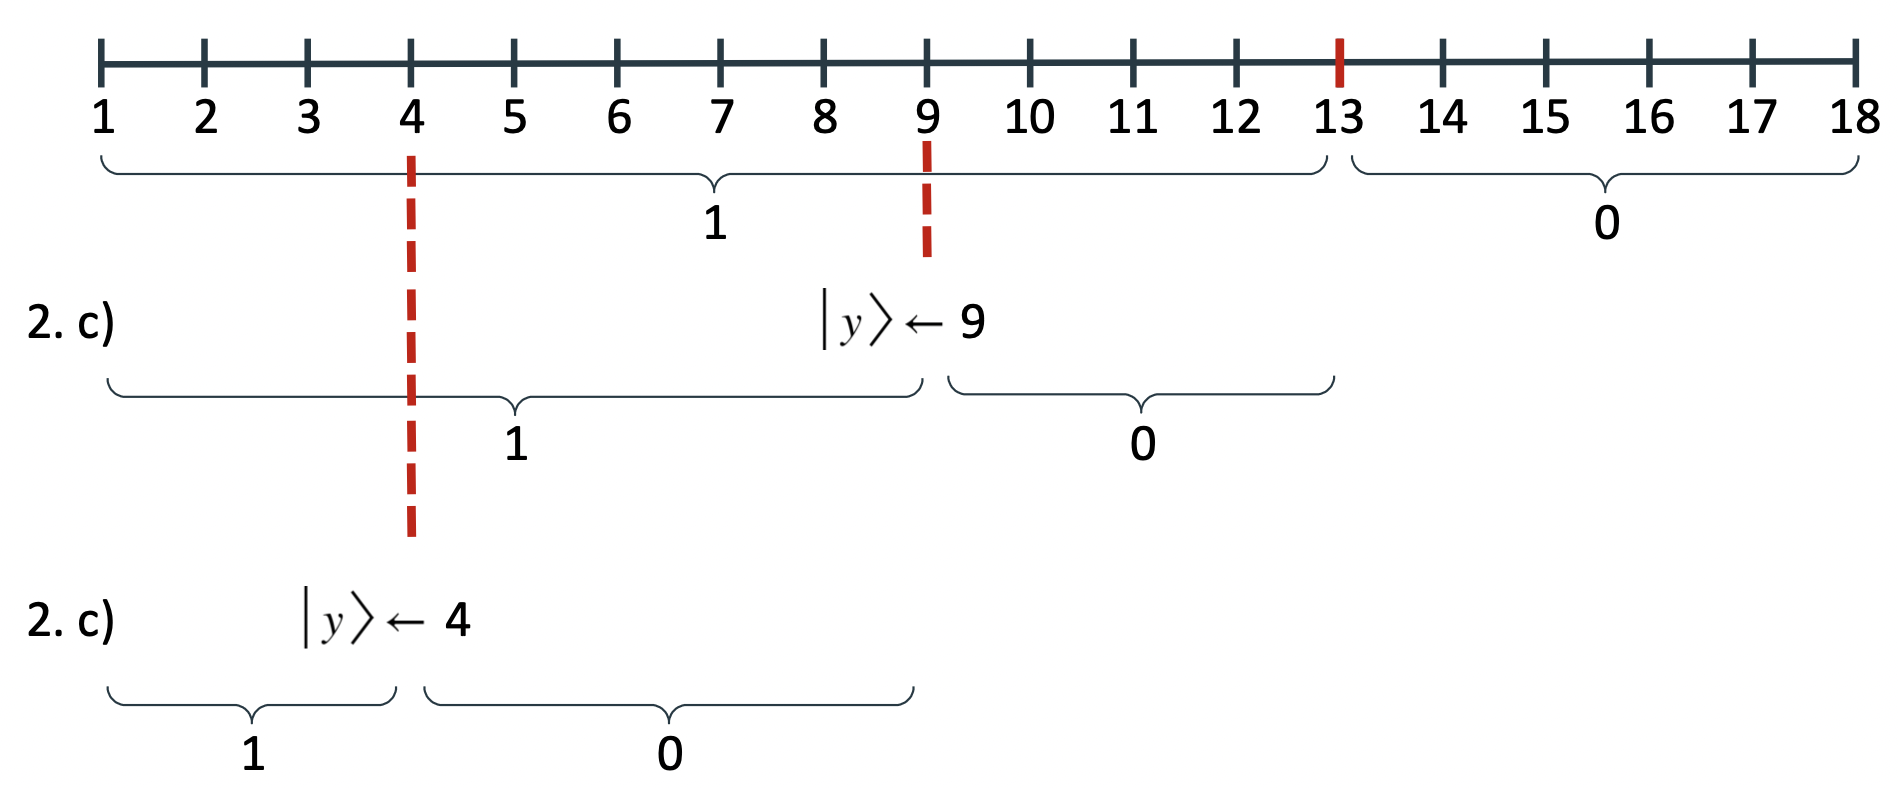
\includegraphics[width=1\textwidth]{figures/suche-minimum-visualisierung.png}}
	\caption{Visualisierung des 2. Schrittes der Suche nach dem Minimum \\ Quelle: Eigene Darstellung}
	\label{fig:sucheMinimumVisualisierung}
\end{figure} 

Mit einer Laufzeit von O LAUFZEIT findet dieser Algorithmus mit über 50\% das minimale Element des Feldes.
